%% LaTeX2e class for student theses
%% sections/evaluation.tex
%% 
%% Karlsruhe Institute of Technology
%% Institute for Program Structures and Data Organization
%% Chair for Software Design and Quality (SDQ)
%%
%% Dr.-Ing. Erik Burger
%% burger@kit.edu
%%
%% Version 1.3.3, 2018-04-17

\chapter{Transformation}
\label{ch:transformation}
Die zuvor vorgestellte Modellierung beschreibt, wie im PCM eine MOM mit expliziten Warteschlangen modelliert und kalibriert werden kann. Wie bereits diskutiert kann eine solche Modellierung sehr aufwändig sein. Ein Architekt muss für einer bestimmte Architektur die Auswirkung verschiedener MOMs untersuchen und vergleichen. Wie bereits beschrieben, stellt das PCM, seit der Arbeit von Rathfelder \cite{Rathfelder2013}, Modellelemente bereit, um eventbasierte Komunikation abzubilden. Bevor eine Performance-Analyse durchgeführt wird, wird eine konkrete Middleware-Architektur in die Architektur eingewoben und die Event-Elemente ersetzt. Der Architekt muss somit nichts an seiner Gesamtarchitektur ändern und tauscht nur die Middleware-Architekturen aus. Ein solcher Ansatz soll auch in dieser Arbeit verwendet werden. Dazu sollen die Event-Elemente beibehalten werden und eine weitere Modelltransformation angeboten werden, um MOMs untersuchen zu können, die Warteschlangen explizit modellieren. Im Folgenden wird beschrieben, wie eine solche Modelltransformation aussehen kann.
%Idee des Event Mechanismus: man moechte konkret ueber nachrichten/events reden und nicht abstrakt ueber interfaces. Event Transformation liefert am Ende Modell mit Interfaces usw. \\
\section{Transformationsprozess}
Zunächst soll beschrieben werden, wie ein solcher Transformationsprozess aussehen soll. Dieser ist in (abb) abgebildet. Der Softwarearchitekt beschreibt im ersten Schritt, wie zuvor auch, die Systemarchitektur und bildet eventbasierte Kommunikation mihilfe der PCM-Event-Elementen ab. Es können auch bereits erstellte Event-Modelle verwendet werden. Im nächsten Schritt muss er sich für eine verfügbare MOM Architektur entscheiden, deren Auswirkung auf das System er untersuchen möchte. Im nächsten Schritt kann er in einer Konfigurationsdatei bestimmte Konfigurationen festlegen. Im Anschluss wird die Systemarchitektur, die ausgewählte MOM und die Konfigurationsdatei mithilfe einer Modeltransformation transfomiert. Im Anschluss dienen die Ergebnissmodelle der Performance-Analyse als Eingabe. Nach Durchführung der Performance-Analyse werden die Ergebnisse dem Architekten bereitgestellt.

\section{Konfiguration der MOM}
Wie bereits in den vorherigen Kapitel beschrieben, haben verschiedene MOMs auch diverse Möglichkeiten konfiguriert zu werden. Damit ein Architekt auch Konfigurationen einer MOM untersuchen kann, soll er in einer Konfigurationsdatei bestimmte Konfigurationen einer MOM angeben können. Diese Konfigurationsdatei ermöglicht es folgendes zu konfigurieren:
\begin{itemize}
    \item Bereitstellen von Warteschlange: Welche Warteschlange wird auf welcher Ressource bereitgestellt. Dabei wird der Name des EventTypes angegeben, welchen die Warteschlange verarbeiten soll. Die Ressource auf der die Warteschlange bereitgestellt werden soll muss vor der Transformation bereits existieren. Außerdem kann Durchsatz und Latenz zu dieser Warteschlange angegeben werden.
    \item Lazy-Warteschlangen: Dabei kann angegeben werden ob die bereitgestellte Warteschlange eine Lazy-Warteschlange ist oder nicht. 
    \item Exchange Zuständigkeit: Dabei kann festgelegt werden welche Warteschlange an welchen Exchange gebunden wird. Dabei kann ein Name für den Exchange und die Namen der dazugehörigen Warteschlangen angegeben werden. Der Name der Warteschlange ist dabei der EventType, welchen die Warteschlange verarbeitet.
    \item Bereitstellen eines Exchange: Auf welcher Ressource wird der Exchange bereitgestellt. Außerdem kann Durchsatz und Latenz zu diesem Exchange angegeben werden.
\end{itemize}
In \autoref{img:configExample} ist eine mögliche Konfigurationsdatei abgebildet. Dabei handelt es sich um eine Xml-Datei. Zu sehen ist, dass es zwei Warteschlangen gibt. Die Erste verarbeitet Nachrichten vom EventType Order. Sie ist wird auf der Ressource Middleware bereitgestellt und ist eine Lazy Warteschlange. Die zweite Warteschlange verarbeitet Nachrichten vom EventType OrderConf. Auch sie wird auf der Ressource Middleware bereitgestellt. Sie ist jedoch keine Lazy-Warteschlange. Beide Warteschlange haben keinen Durchsatz und Latenz angegeben. Außerdem gibt es nur einen Exchange. Dieser wird ebenfalls auf der Middleware Ressource bereitgestellt. Er hat einen Durchsatz in Bytes und eine Latenz in ms angegeben. Die von ihm verwalteten Warteschlangen sind die beiden zuvor definierten Warteschlangen.

\begin{figure}
\center
  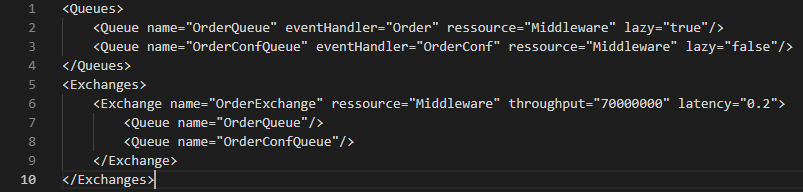
\includegraphics[width=1\textwidth]{code/configExample.png}
  \caption{beispiel einer Kommunikation in RMQ}
  \label{img:configExample}
\end{figure}

\section{Generierung von Exchange und Warteschlangen}
Im Ersten Schritt werden im Repository-Modell Exchange Komponenten eingefügt. Dabei wird die Anzahl und die Namen aus der Konfigurationsdatei ausgelesen. Außerdem werden die Ressourcen Anforderungen für Latenz und Durchsatz an die passende Stelle, des jeweiligen Exchange, eingesetzt. Diese wurden in \autoref{sec:kalibrierung} beschrieben. Die Komponenten werden wie im vorherigen Kapitel angeboten. Im nächsten Schritt wird jeder Sender identifiziert, der ein EventType aussendet. Für diese Sender werden jeweils eine requiredRole eingefügt, die einen der zuvor eingefügen Exchanges benötigt. Dabei werden die EventTypes beachtet. Jede EmitAction eines Senders wird nun durch einen ExternalCall ersetzt, der im jeweiligen Exchange die Funktion Exchange.distribute aufruft. Als Parameter wird eine UsageVariable mitgegeben, die als Typ den Namen der zuvor aussendenden EventAction hat. Außerdem wird eine Warteschlangen Komponente angelegt die Nachrichten vom Typ EventType.name entgegen nimmt. Bei der Erstellung werden außerdem passende Ressourcen Anforderungen für eine Nachricht eingefügt. Diese werden aus der Konfigurationsdatei entnommen und an die passenden Stellen eingesetzt. Dies wurde in \autoref{sec:kalibrierung} beschrieben. In dem jeweiligen Exchange, der für diesen EventType zuständig ist, wird eine requiredRole eingefügt, die diese Warteschlange benötigt. Als nächstes wird in den distribute Seff des Exchange ein guardedBranch eingefügt. Die Bedingung lautet Type == EventType.name. Im Anschluss wird eine ExternalCallAction eingefügt die die Queue.put Funktion in der zuvor erstellten Warteschlange aufruft. Nachdem alle Sender abgearbeitet wurden, wird nach allen Empfängern gesucht, die einen EventType handhaben. Zunächst wird für diesen EventType ein Interface der Form IRecvX, mit X = EventType.name angelegt. Dieses Interface hat eine Signatur der Form recvX. Dieses Interface wird von dem aktuell betrachteten Empfänger angeboten. Außerdem wird eine requiredRole erstellt, die den Exchange benötigt, der dem EventType zugeordnet ist. Ein Seff wird erstellt, der die Funktionalität von IRecvX.recvX abbilden soll. Dieser enthält einen ExternalCallAction, die die Exchange.receive im benötigten Exchange aufruft mit einer UsageVariable mit Type=EventType.name als Parameter. Als nächstes wird im receive Seff des Exchange ein guardedBranch eingefügt. Die Bedingung lautet Type == EventType.name. Im Anschluss wird eine ExternalCallAction eingefügt die die Queue.get Funktion in der Warteschlange aufruft, die Nachrichten vom Typ EventType beinhalten. Im Anschluss werden die Event-Elemente aufgeräumt.

TODO Bild


\section{Transformation von Punkt-Zu-Punkt Kommunikation}
Im Folgenden wird beschrieben, wie die Punkt-Zu-Punkt Kommunikation zwischen Komponenten transformiert wird. Dabei wird das System- und Nutzungsmodell transformiert. Als erster Schritt werden die zuvor erstellen Exchange und Warteschlangen Komponenten im Systemmodell in einem AssemblyContext eingefügt. Im Anschluss werden alle Warteschlangen mit dem jeweiligen Exchange über die passende Schnittstelle mit einem AssemblyConnector verbunden. Als nächstes werden alle AssemblyEventConnectoren gesucht. Jeder AssemblyEventConnector hat ein SourceRole und ein SinkRole Feld. Für jede SourceRole wird die darin enthaltene Komponente über einen AssemblyConnector mit dem Exchange verbunden. Die Komponente die sich im SinkRole Feld befindet wird ebenfalls mit dem Exchange mithilfe eines AssemblyConnector verbunden. Außerdem wird für jede dieser SinkRole-Elemente eine SystemProvidedRole erstellt. Die SinkRole Komponente und die SystemProvidedRole werden mit einem DelegationsConnector verbunden. Schließlich wird im Nutzungsmodell eine UsageScanrio angelegt um das abholen von Nachrichten abzubilden. Dazu wird in dem UsageScenario ein EntryLevelSystemCall angelegt, der über die jeweilige SystemProvidedRole Exchange.receive aufruft. Außerdem wird ein ClosedWorkload mit Population eins und einer ThinkTime von null angelegt.

TODO Bild

TODO Aufräumen der Event Elemnte

\section{Transformation von Viele-Zu-Viele Kommunikation}
Im Fall von Viele-Zu-Viele Kommunikation werden neben dem System- und Nutzungsmodell auch das Repository-Modell angepasst. Die Viele-Zu-Viele Kommunikation findet im PCM über einen EventChannel statt. Sender sind über eine SourceConnector und Empfänger über einen SinkConnector mit diesem verbunden. Für jeden SourceConnector, der die Sender Komponente mit dem EventChannel verbindet, wird eine AssemblyConnector zwischen dem Sender und dem jeweiligen Exchange erstellt. Bei der Transformation der SinkConnectoren wird zunächst ein neuer AssemblyContext mit Warteschlagen Komponente erstellt. Im Repository-Modell wird im Exchange eine neue RequiredRole angelegt die diese Warteschlange benötigt angelegt. Im distribute Seff wird der guardedBranch erweitert, der das dazugehörige Event behandelt. Für die zuvor erstellte RequiredRole wird ein weiterer ExternalCallAction erstellt, der die Nachricht an die Warteschlange sendet. Somit wird die Nachricht an mehrere Wartschlangen weitergeleitet. Im Systemmodell wird mit einem AssemblyConnector der Exchange und die Warteschlange verbunden. Außerdem wird für den Empfänger AssemblyContext eine SystemProvidedRole erstellt und mit dem AssemblyContext mithilfe eines DelegationsConnector verbunden. Schließlich wird wie auch bei der Punkt-Zu-Punkt Transformation, im Nutzungsmodell eine UsageScanrio angelegt. Damit soll das abholen von Nachrichten ab gebildet werden. In dem UsageScenario wird ein EntryLevelSystemCall angelegt, der über die jeweilige SystemProvidedRole Exchange.receive aufruft. Außerdem wird ein ClosedWorkload mit Population eins und einer ThinkTime von null angelegt.


TODO Bild

TODO Aufräumen der Event Elemnte

\section{Bereitstellen der Komponenten}
Das bereitstellen der Komponenten setzt voraus, dass in der vom Benutzer angegebenen Konfiguration festgelegt wurde, welche Warteschlange und welcher Exchange auf welcher Ressource bereitgestellt werden soll. Diese Ressourcen müssen bereits vor der Transformation erstellt worden sein. Währende der Transformation werden die Komponenten auf den Ressourcen im Allokations-Modell bereitgestellt. Dazu wird ein AllocationContext erstellt und der AssemblyContext mit der dazugehörigen Ressource bereitgestellt.

